% !TeX spellcheck = hu_HU
% !TeX encoding = UTF-8
\newcommand{\plotscale}{0.6}

\chapter{Kiértékelés} \label{sec:kiertekeles}
\section{Adatbázis-kezelő rendszerek teljesítményének mérése az LDBC SNB keretrendszerrel}
\subsection{Motiváció}

Bár a relációs adatbázis-kezelők a mai napig a legelterjedtebb adatbázis-kezelők\footnote{\url{https://db-engines.com/en/ranking}}, az újgenerációs adatbázis-kezelők változatos funkcionalitásaikkal és lekérdezőnyelveikkel újra és újra megpróbálják felvenni a versenyt velük. A gráf alapú adatbázis-kezelők az utóbbi években jelentős fejlődésen mentek keresztül, ezzel jelentősen növelve népszerűségüket\footnote{\url{https://db-engines.com/en/ranking_categories}}. Ahhoz, hogy eldöntsük, fel tudják-e venni a versenyt a relációs adatbázis-kezelőkkel, szükséges a teljesítményük összehasonlítása is. 

A dolgozatban összehasonlított alkalmazások összetettsége bőven meghaladja azt a szintet, hogy a teljesítményüket a forráskódok elemzése alapján össze lehetne hasonlítani. Ezért a tudományban már bizonyított módon kísérletek, mérések alapján próbálom összehasonlítani őket.

A dolgozatban összehasonlított technológiák kiválasztásában leghangsúlyosabb szempont a lekérdezőnyelveik voltak:
\begin{itemize}
	\item SQL: Régóta használt, a legelterjedtebb relációs adatbázis-kezelők szabványos nyelve.
	\item SPARQL: A dolgozatban bemutatott gráf alapú lekérdezőnyelvek közül a legteljesebb matematikai háttérrel rendelkező, szemantikailag legtisztább lekérdezőnyelv.
	\item Cypher: A gráf alapú lekérdezőnyelvek között az egyik legnépszerűbb lekérdezőnyelv, véleményem szerint az egyik legintuitívabb és legkifejezőbb nyelv.
\end{itemize}

\begin{table}[h]
	\centering
	\begin{tabular}{|l|r|r|r|}
		\toprule
		\multicolumn{1}{l}{Nyelv} & \multicolumn{1}{l}{BI karakterszám} & \multicolumn{1}{l}{Int. karakterszám}& \multicolumn{1}{l}{Összesen} \\
		\midrule
		Cypher & 13\,657 & 19\,021 & 32\,678 \\
		SPARQL & 32\,417 & 43\,548 & 75\,965 \\
		SQL    & 30\,417 & 14\,563 & 44\,980 \\
		\bottomrule
	\end{tabular}
	\caption{A különböző nyelveken megírt BI és Interactive lekérdezések karakterszáma fehér szóközök (szóközök, tabulátor és újsor karakterek) nélkül}
	\label{tab:char-count}
\end{table}

A Cypher kifejezőerejét és tömörségét \aref{tab:char-count}.~táblázat is alátámasztja. A lekérdezések SQL-ben 37\%, SPARQL-ben pedig 132\%-kal több karaktert tartalmaznak, mint a Cypherben írt lekérdezések.

Annak érdekében, hogy átfogó képet kapjak az elérhető gráf információs rendszerek teljesítményéről, egy összetett mérési sorozatot terveztem és futtattam.

\subsection{Business Intelligence terhelési profil}

A mérés során három implementációval végeztem méréseket a BI terhelési profil felhasználásával:

\begin{enumerate}
	\item PostgreSQL: a PostgreSQL relációs adatbázis-kezelő rendszer.
	\item Sparksee: a Sparksee tulajdonsággráf adatbázis-kezelő rendszer.
	\item \stardog: egy szemantikus adatbázis.
\end{enumerate}

A meg nem nevezett adatbázis-kezelő rendszer eredményeit anonimizált módon adom közre. Ennek oka, hogy ugyan a lekérdezések minden esetben \emph{validáltak} (azaz helyes eredményeket biztosítanak), de nem \emph{auditáltak} (azaz a rendszerek gyártói nem vizsgálták meg az implementációt, így nem garantált, hogy az optimális teljesítményt biztosít).

A teljesítménymérés során az egyes implementációk válaszidejét és skálázhatóságát mértem. Válaszidő alatt a lekérdezés végrehajtásának elkezdésétől a lekérdezésre adott válasz teljes megérkezéséig eltelt időt értjük. A skálázhatóság alatt a válaszidő adathalmaz méretétől függő változását értem. 

\subsubsection{Mérési elrendezés}

A dolgozat készítése során végzett mérések egy számítógépen történtek az LDBC SNB keretrendszer driver szoftvermoduljának 0.3.1-es verziójának felhasználásával. A számítógép 8 fizikai processzormagot (Intel(R) Xeon(R) E5-2673), és 256 GB memóriát tartalmaz. A háttértár egy SCSI interfészen kapcsolt 128GB-os SSD lemez. Az operációs rendszere 64 bites Ubuntu 16.04.

A PostgreSQL 10.5-ös verzióját használtam az SQL mérésére. A meg nem nevezett adatbázis-kezelő méréséhez az utóbbi 6 hónapban kiadott verziót használtam. A driver és opcionálisan a meg nem nevezett adatbázis-kezelő rendszer az OpenJDK 1.8.0\_181-es verzióját használták. Az adatbázis-kezelő konfigurációját a dokumentációja alapján próbáltam optimalizálni, azonban az anonimitás miatt a pontos beállításokat nem közölhetem.

A lekérdezések \aref{sec:keretrendszer}.~fejezetben leírt módon kerültek ellenőrzésre az SF1-es adathalmazokon.
A teljesítménymérés során a rendszereken először futtattam 100 darab bemelegítő (warmup) lekérdezést, majd 250 lekérdezés válaszidejét mértem meg. A lekérdezések véletlenszerűen választottak és végrehajtásuk szekvenciálisan, átlapolódás nélkül történt. 

\begin{figure}
	\centering
	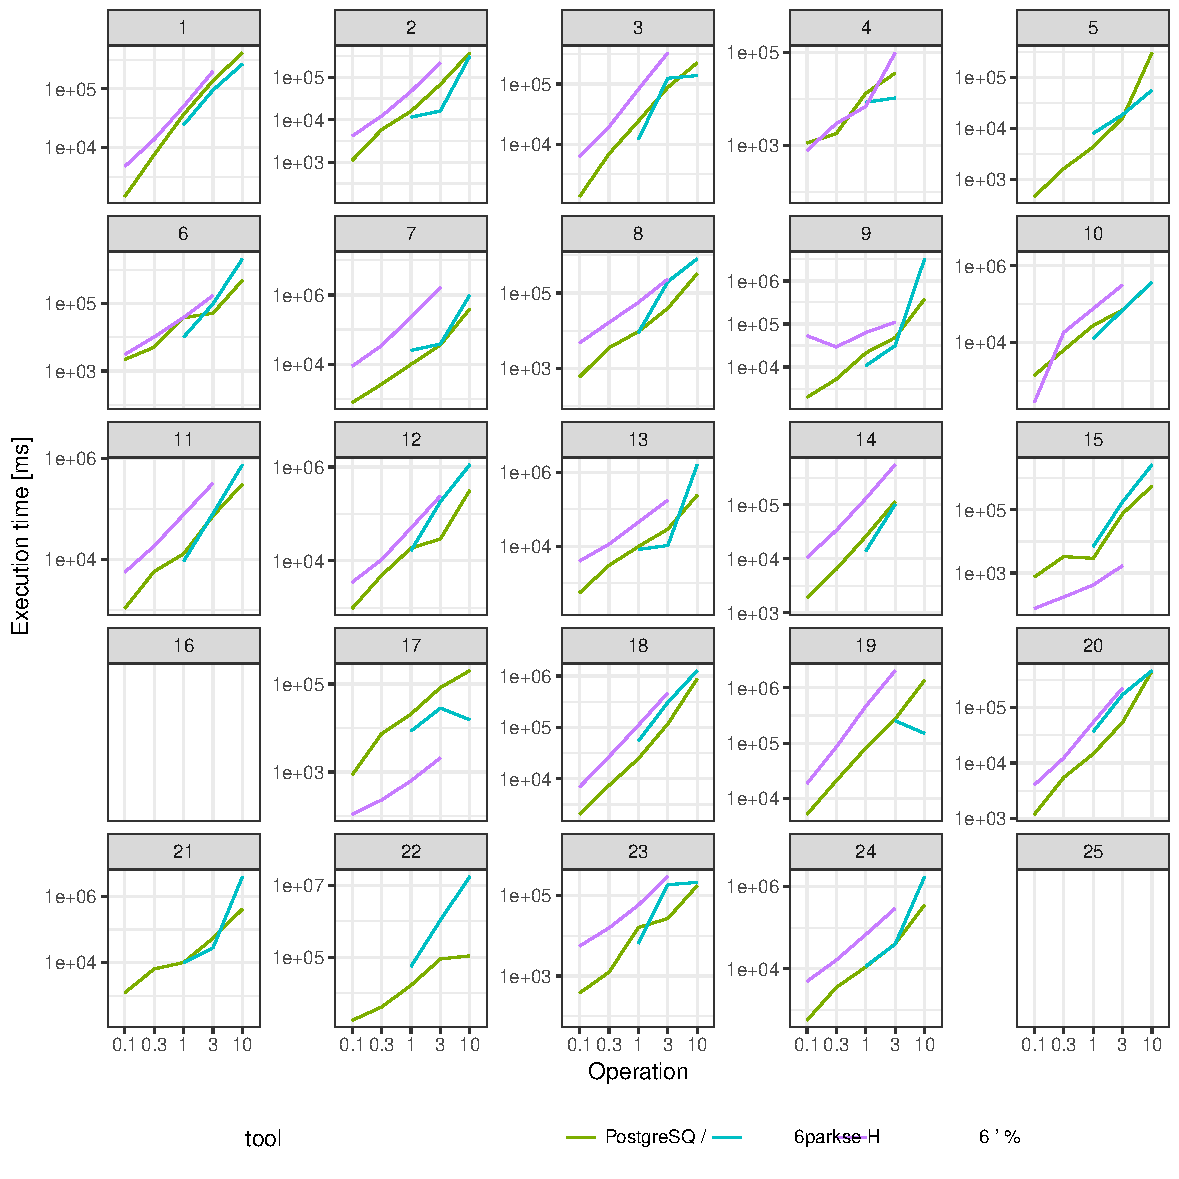
\includegraphics[width=\textwidth]{bi-execution-times}
	\caption{A lekérdezések összesített mérési eredményei}
	\label{fig:bi-execution-times}
\end{figure}

\subsubsection{Eredmények értékelése}

A mérési eredményeket \aref{fig:bi-execution-times}.~ábra tartalmazza. A profil bonyolultságát jól szemlélteti, hogy több olyan lekérdezést (4-es és 14-es) is tartalmaz, amelyeket egyik adatbázis-kezelő sem tudott végrehajtani a legnagyobb adathalmazon, továbbá számos lekérdezés válaszideje elérte a több tíz másodpercet mindhárom rendszer esetében már az SF3-as adathalmazon is (1-es, 3-as, 11-es, 14-es, 15-ös, 18-as, 19-es, 22-es lekérdezés). Egyértelműen látszik, hogy nehezebben megfogalmazható és összetettebb lekérdezéseket tartalmaz, mint az Interactive profil.

Érdemes megfigyelni, hogy a Sparksee két lekérdezés (17-es és 19-es) esetében is jobb válaszidőt produkált az SF10-es adathalmazon, mint az SF3-as adathalmazon.

\subsection{Interactive terhelési profil}
A mérés során négy implementációval végeztem méréseket az Interactive terhelési profil komplex lekérdezéseinek felhasználásával:

\begin{enumerate}
	\item PostgreSQL: a PostgreSQL relációs adatbázis-kezelő rendszer.
	\item Sparksee: a Sparksee tulajdonsággráf adatbázis-kezelő rendszer.
	\item \virtuoso: egy szemantikus adatbázis.
	\item \stardog: egy szemantikus adatbázis.
\end{enumerate}

A két meg nem nevezett adatbázis-kezelő rendszer eredményeit a BI terhelési profilhoz hasonlóan anonimizált módon adom közre a már említett ok miatt: a lekérdezések \textit{validáltak}, de nem \textit{auditáltak}.

A teljesítménymérés során az egyes implementációk válaszidejét és skálázhatóságát mértem. Válaszidő alatt a lekérdezés végrehajtásának elkezdésétől a lekérdezésre adott válasz teljes megérkezéséig eltelt időt értjük. A skálázhatóság alatt a válaszidő adathalmaz méretétől függő változását értjük. 

\subsubsection{Mérési elrendezés}

A dolgozat készítése során végzett mérések egy számítógépen történtek az LDBC SNB keretrendszer driver szoftvermoduljának 0.3.1-es verziójának felhasználásával. A számítógép 16 fizikai processzormagot (Intel(R) Xeon(R) Platinum 8167M CPU @ 2.00GHz), és 236 GB memóriát tartalmaz. A háttértár egy SCSI interfészen kapcsolt 128GB-os SSD lemez. Az operációs rendszere 64 bites Ubuntu 18.04.

A PostgreSQL 10.5-ös\footnote{(PostgreSQL 10.5 (Ubuntu 10.5-0ubuntu0.18.04) on x86\_64-pc-linux-gnu, compiled by gcc (Ubuntu 7.3.0-16ubuntu3) 7.3.0, 64-bit)} verzióját használtam az SQL implementációk mérésére.

A meg nem nevezett adatbázis-kezelők méréséhez (a BI profil méréséhez hasonlóan) az utóbbi 6 hónapban kiadott verziókat használtam. A driver és a meg nem nevezett adatbázis-kezelők közül a Java nyelvű rendszerek az OpenJDK 1.8.0\_181-es verzióján futottak. Az adatbázis-kezelők konfigurációját a dokumentációjuk alapján próbáltam optimalizálni, azonban az anonimitás miatt a pontos beállításokat nem közölhetem.

A lekérdezések a rövid lekérdezésekkel és a frissítésekkel együtt \aref{sec:keretrendszer}.~fejezetben leírt módon kerültek ellenőrzésre az SF1-es adathalmazokon, több mint 13 ezer lekérdezés eredményének összehasonlításával.

\begin{table}
	\centering
	\begin{tabular}{|l|r|r|r|}
		\toprule
		Skálázási tényező & SF1 & SF3 & SF10 \\
		\midrule
		PostgreSQL & 1000 & 1000 & 1000 \\
		Sparksee & 1000 & 1000 & 1000 \\
		\virtuoso & 1000 & 1000 & 1000 \\
		\stardog & 1000 & 750 & 40 \\
		\bottomrule
	\end{tabular}
	\caption{A implementációk mérése során futtatott lekérdezések száma}
	\label{tab:query-count}
\end{table}

A mérés során a lekérdezéseket különböző behelyettesítési paraméterekkel futtattam \aref{tab:query-count}.~táblázat szerinti darabszámban. Annak érdekében, hogy a mérések összideje ne legyen túl nagy, több korlátozást is kellett tennem. A \stardog mérése során már SF3 esetében is csökkenteni kellett a lekérdezések számát, illetve az SF10-es adathalmazon egyáltalán nem mértem le az \stardog-t, mert nem futott le egy lekérdezés sem.

Mindegyik eszköz mérésnél a különböző méretű adathalmazokon legalább 20-szor futott egy lekérdezés (különböző paraméterekkel).


\subsubsection{Eredmények értékelése}

A mérési eredményeket \aref{fig:results-interactive-aggregated}.~ábra tartalmazza.

\begin{figure}
	\centering
	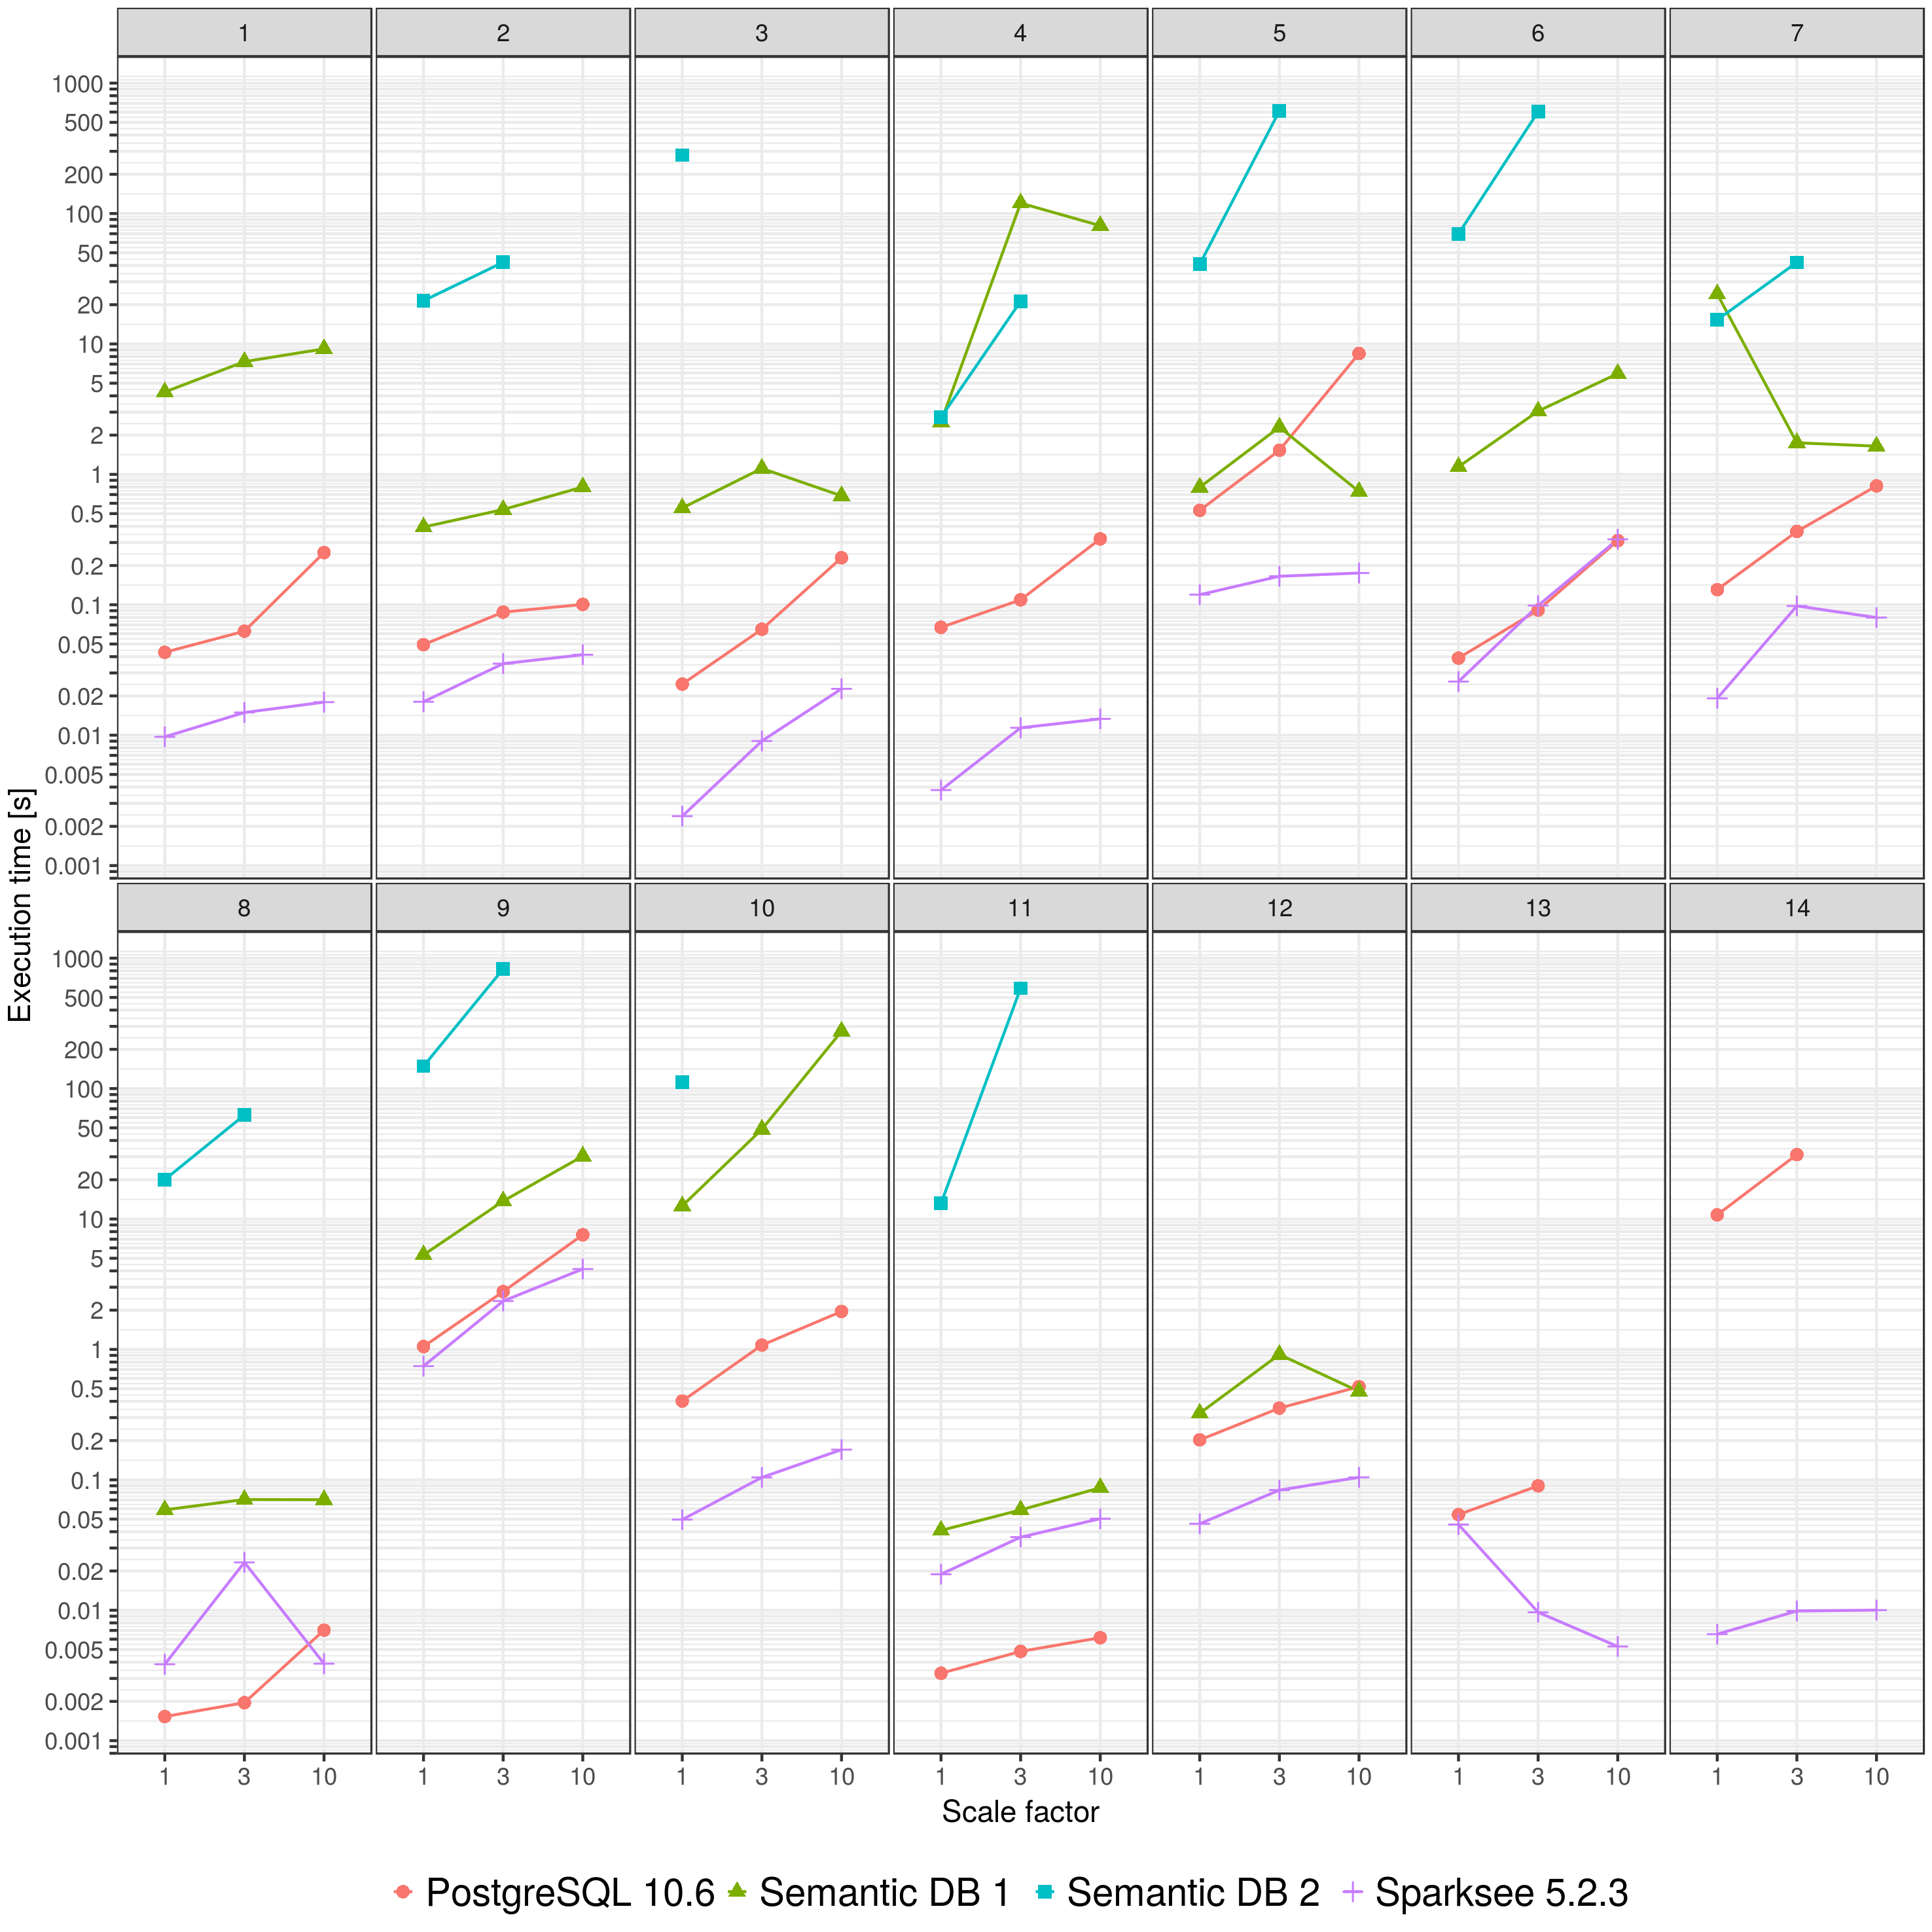
\includegraphics[scale=\plotscale]{results/results-interactive-aggregated.png}
	\caption{A lekérdezések összesített mérési eredményei}
	\label{fig:results-interactive-aggregated}
\end{figure}

Az egyik legfontosabb eredmény, hogy a lekérdezések többségénél a legjobb eredményt a Sparksee érte el. Hozzá hasonlóan jól teljesített a PostgreSQL, ezzel bizonyítva, hogy a relációs adatbázis-kezelők a közel 50~éves fejlődésnek köszönhetően manapság is a leghatékonyabb adatbázis-kezelők közé tartoznak.

Megfigyelhető, hogy a 3-as, 4-es, 5-ös és 12-es lekérdezéseknél az \virtuoso eszköz kisebb átlagos válaszidővel rendelkezik az SF10-es adathalmazon, mint az SF3-as adathalmazon. A lekérdezések specifikációjából~\cite{LDBC_SNB} kiderül, hogy az említett lekérdezésekben szerepel összetett aggregáció. Az említett lekérdezéseken kívül összetett aggregáció csak a 6-os lekérdezésben van, amelynél azonban nem figyelhető meg ilyen fajta teljesítmény-növekedés. A jelenségre nem sikerült konkrét hipotézist felállítani, de az említett komplex aggregációnak köze lehet a jelenséghez.

A 7-es lekérdezésnél szintén megfigyelhető a teljesítmény javulása a nagyobb adathalmazokon. Abban azonban más jellegű ez a javulás, mert az SF1 adathalmaz után, az SF3-as adathalmaznál figyelhető meg jelentős javulás, míg az SF3 adathalmaz után az SF10-es adathalmaznál csak minimális mértékű.

\begin{figure}
	\centering
	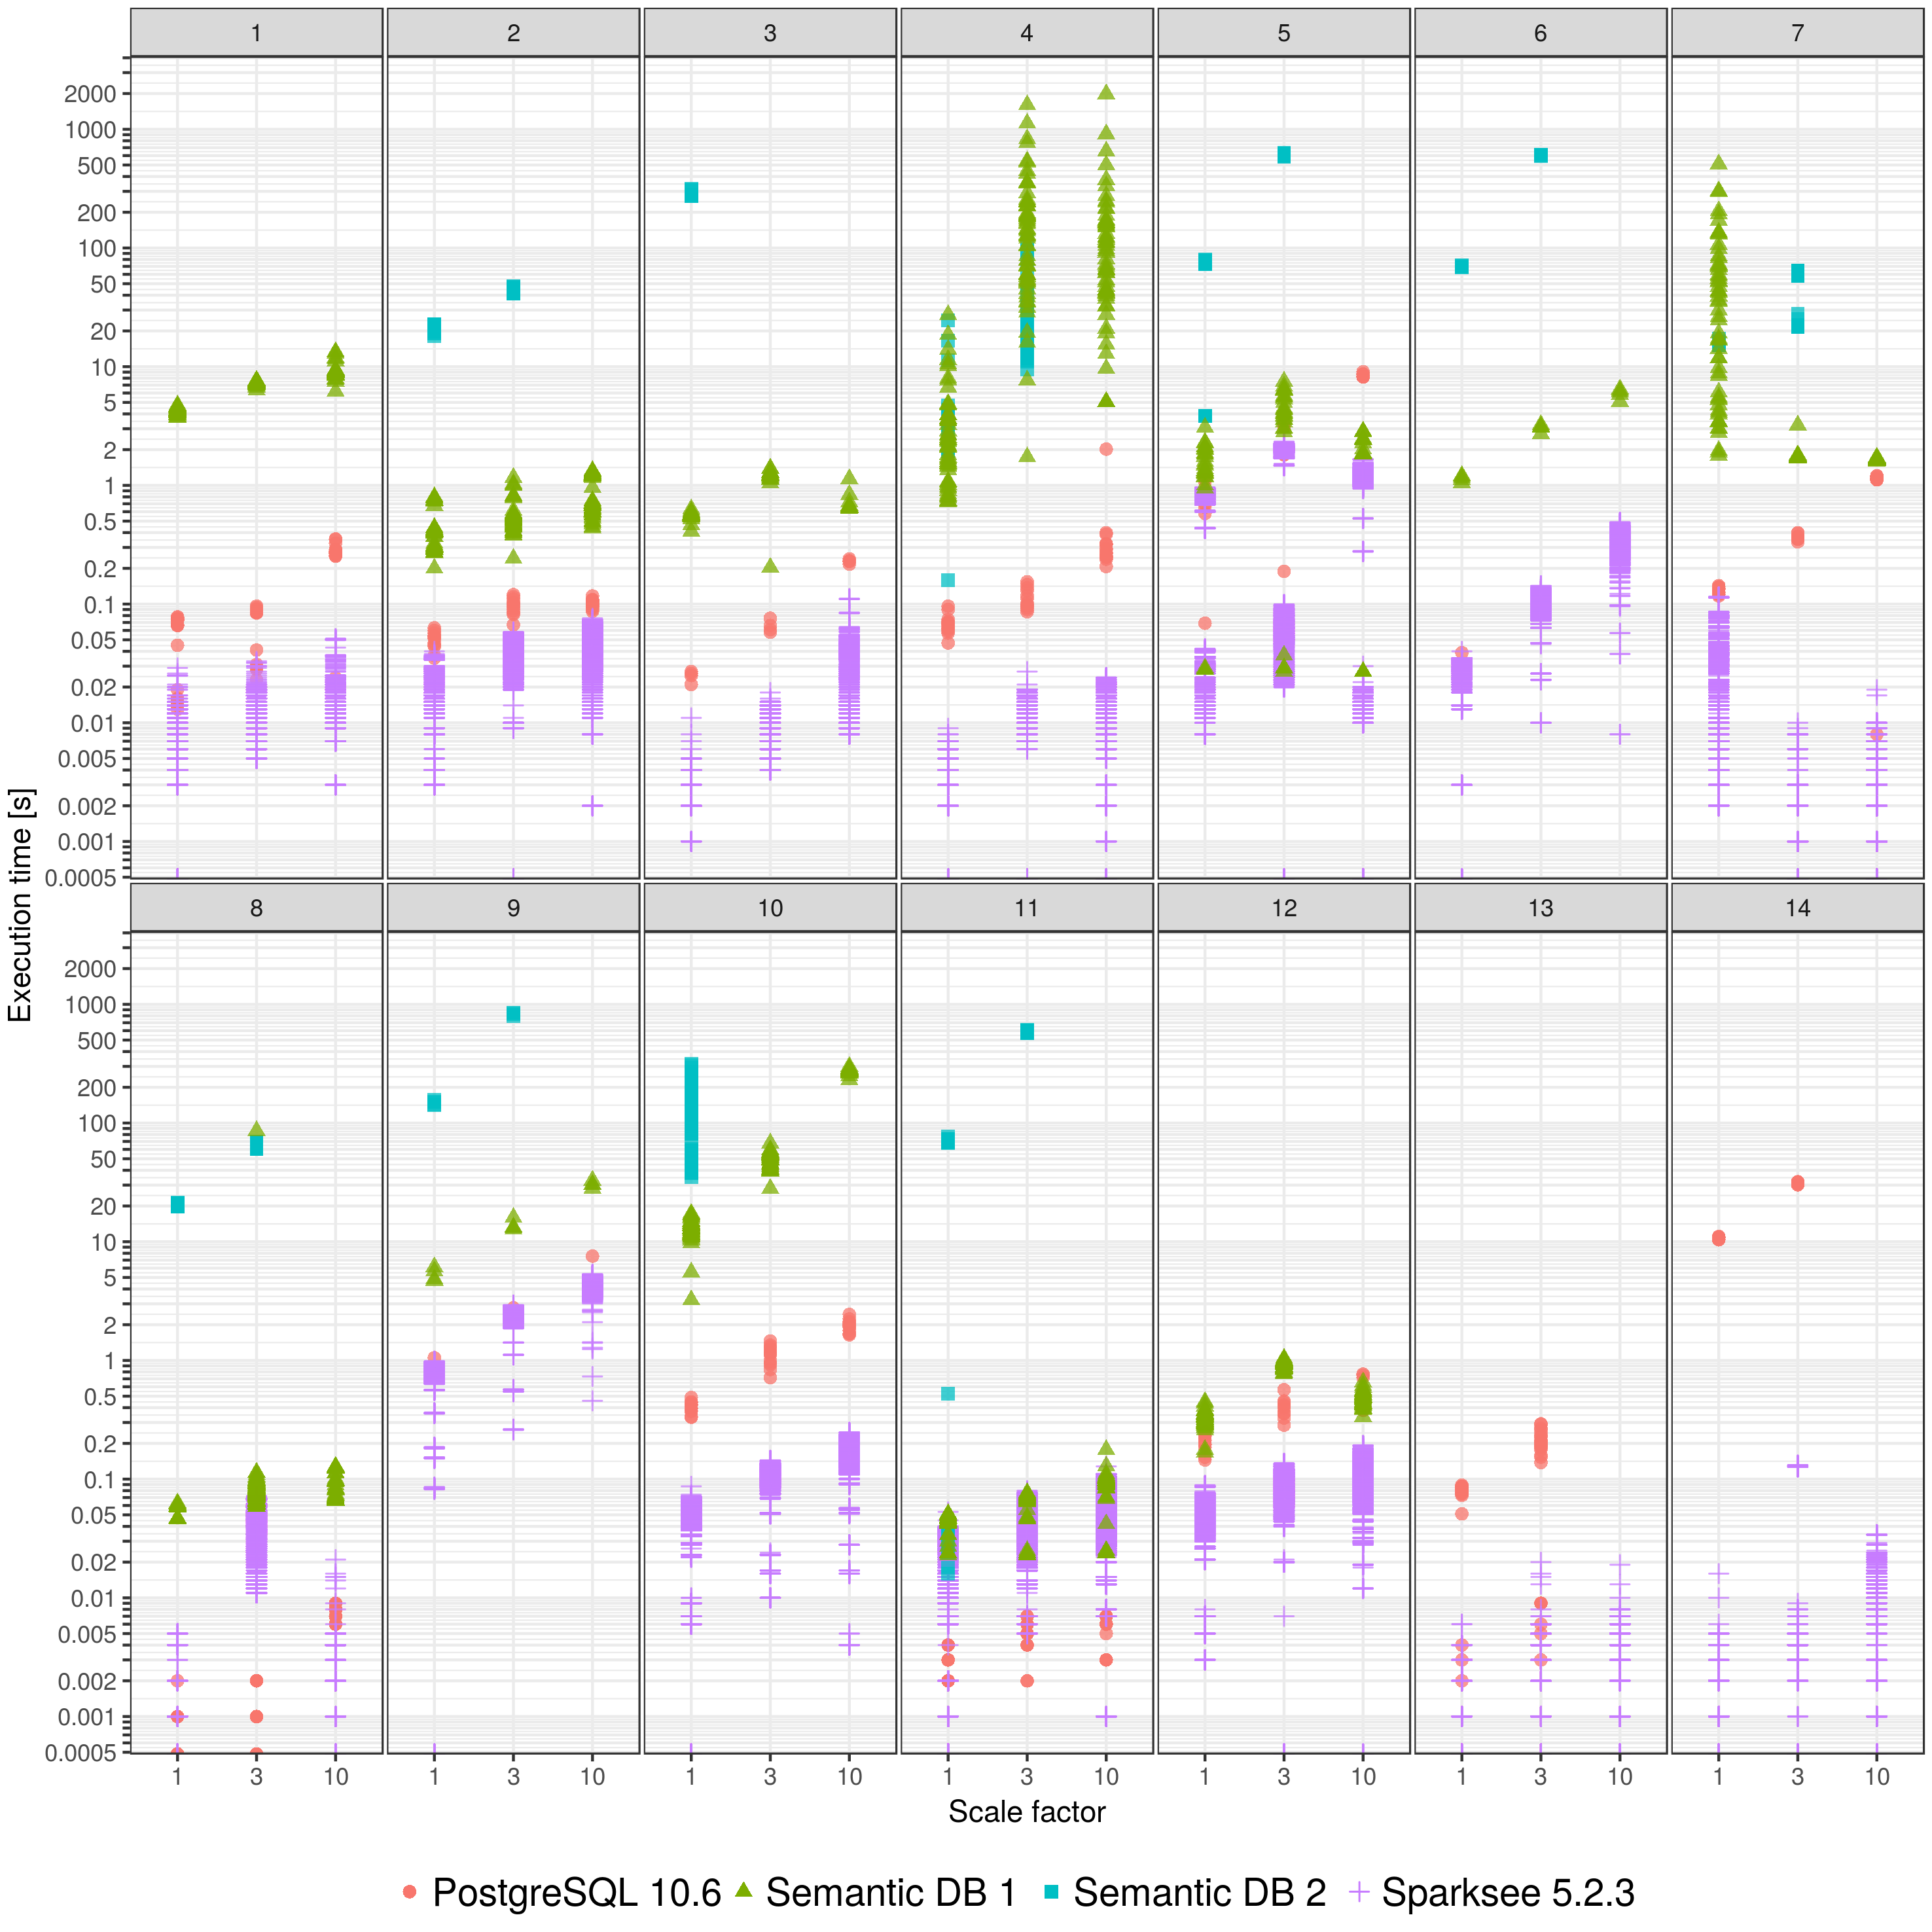
\includegraphics[scale=\plotscale]{results/results-interactive-detailed.png}
	\caption{A lekérdezések részletes mérési eredményei}
	\label{fig:results-interactive-detailed}
\end{figure}

A lekérdezések részletesebb eredményeit ábrázolja \aref{fig:results-interactive-detailed}.~ábra. Megfigyelhető, hogy az eszközök egy adott lekérdezés esetében is nagyságrendekkel eltérő válaszidővel rendelkezhetnek a lekérdezés paramétereitől függően. Kifejezetten látványos az \virtuoso viselkedése a 4-es lekérdezés esetében, ahol a legjobb és a legrosszabb eredmény között több, mint két nagyságrendnyi az eltérés.

Hasonlóan érdemes megvizsgálni a Sparksee viselkedését az 5-ös lekérdezés esetében. A mérési eredmények mindhárom méretű adathalmazon két jól elkülöníthető csoportba sorolhatóak: \textit{(1)} az 1 tizedmásodperc alatti és az \textit{(2)} egy másodperc körüli válaszidők csoportjába. Előbbiekre lehetséges magyarázat lehetne az, hogy a lekérdezés ebben az esetben üres eredményhalmazt ad vissza, de tapasztalataim szerint ez nem igaz.

Az említett jelenségek többségére sajnos hipotéziseket sem tudtam felállítani. Ennek egyik oka, hogy a rendszerek belső működéséről nincs információm, ezért nem tudok következtetni a lehetséges okokra.

\section{Differenciális adatfolyamok teljesítménymérése TTC-vel}

\subsection{Motiváció}

A DAF számítási modell pozitív tulajdonságai miatt (elosztott, nagy teljesítményű, iteratív és inkrementális számítások támogatása) a hatékony INK egyik lehetséges megoldása lehet. A gráfadatbázisokban való felhasználásához azonban fontos tisztában lenni azzal, hogy a gráf alapú adathalmazokon milyen teljesítményt nyújt. Ez a cél tökéletesen illeszkedik a TTC 2018-as versenyfeladatához, ahol a cél az, hogy minél jobb teljesítményű (skálázódás és válaszidő szempontjából is) megoldást készítsünk. Ezért elkészítettem a feladat megoldását a Naiad szoftverkönytár által nyújtott DAF keretrendszerrel, teljesítményét pedig összehasonlítottam a többi megoldás teljesítményével. Így a mérés során az alábbi eszközök teljesítményét hasonlítottam össze:
\begin{itemize}
	\item DAF implementáció a Naiad könyvtár használatával, 1, 2, 4, 6 és 8 szálon történő feldolgozással
	\item NMF alapú inkrementális megoldás
	\item \viatra alapú inkrementális megoldás
	\item Xtend nyelven\footnote{\url{https://www.eclipse.org/xtend/}} manuálisan megvalósított inkrementális megoldás
\end{itemize}
Az Xtend egy Java forráskódra forduló programozási nyelv. Szintaxisa nagyon hasonló a Java nyelvhez, azonban számos szintaktikai édesítőszerrel egészíti ki annak szintaxisát.

\subsection{Mérési elrendezés}\label{sec:naiad-layout}

A méréseket egy számítógépen végeztem el a TTC által nyújtott keretrendszer használatával. A számítógép 6 fizikai processzormagot (Intel Core i7-8700K @ 3.70GHz) és 32 GB memóriát tartalmaz. A háttértár SATA2 interfészen csatolt 512GB-os SSD lemez. Az operációs rendszer 64 bites Windows 10.

A Java környezetből az Oracle Java 8u191-es, a .NET Core 2.2-es és a .NET Framework 4.7.2-es verzióját használtam a mérés során. Az eszközök mérése során a különböző adathalmazokon 3-szor futtattam minden eszközt, az eredményeket aggregáltam az értékek mértani közepét (geometric mean) véve, \cite{DBLP:journals/cacm/FlemingW86} javaslatának megfelelően. Egy futtatás alkalmával a TTC által az adott modellhez tartozó összes (20 darab) frissítést végrehajtottam és a modell betöltése és minden frissítés után lefuttattam a mért lekérdezést. A két lekérdezés mérése szekvenciálisan, átlapolódás nélkül történt történt.

A mérés során használt modelleket egy számmal azonosítjuk. A modellek számozása megegyezik a 2 hatványaival, mivel a legkisebb modellt önkényesen 1-gyel jelölték és a modellek mérete nagyjából duplázódik. A modellek legfontosabb jellemzőit \aref{tab:ttc-modells}.~táblázat mutatja be.
\begin{table}[h]
	\centering
	\begin{tabular}{rrrrr}
		\toprule
		\multicolumn{1}{l}{Modell} & \multicolumn{1}{l}{Felhasználók} & \multicolumn{1}{l}{Bejegyzések}& \multicolumn{1}{l}{Hozzászólások} & \multicolumn{1}{l}{Méret (MB)} \\
		\midrule
		1 & 80 & 554 & 638 & 0.154 \\
		2 & 118 & 889 & 1\,059 & 0.252 \\
		4 & 190 & 1\,845 & 2\,305 & 0.538 \\
		8 & 204 & 2\,270 & 5\,027 & 0.984 \\
		16 & 394 & 5\,518 & 9\,136 & 2.1 \\
		32 & 595 & 10\,929 & 18\,689 & 4.3 \\
		64 & 781 & 18\,083 & 38\,753 & 8.3 \\
		128 & 1\,158 & 37\,228 & 75\,605 & 18 \\
		256 & 1\,678 & 74\,668 & 145\,821 & 34 \\
		512 & 2\,606 & 167\,299 & 267\,160 & 68 \\
		1\,024 & 3\,699 & 314\,510 & 526\,006 & 136 \\
		\bottomrule
	\end{tabular}
	\caption{Az egyes modellekben szereplő modellelemek darabszáma (db) és a kezdeti modell mérete MB-ban}
	\label{tab:ttc-modells}
\end{table}

A \viatra és Xtend alapú megoldásokat nem mértem a nagyobb adathalmazokon, mivel a teljesítménymérés túl hosszú ideig tartott volna.

\subsubsection{Eredmények értékelése}

Az eredmények értékelésénél fontos kiemelni, hogy a mért lekérdezések validáltak, de nem auditáltak (azaz az eszközök fejlesztői által nem vizsgáltak, így nem garantált, hogy optimális teljesítményt nyújtanak).

\begin{figure}[ht!]
	\centering
	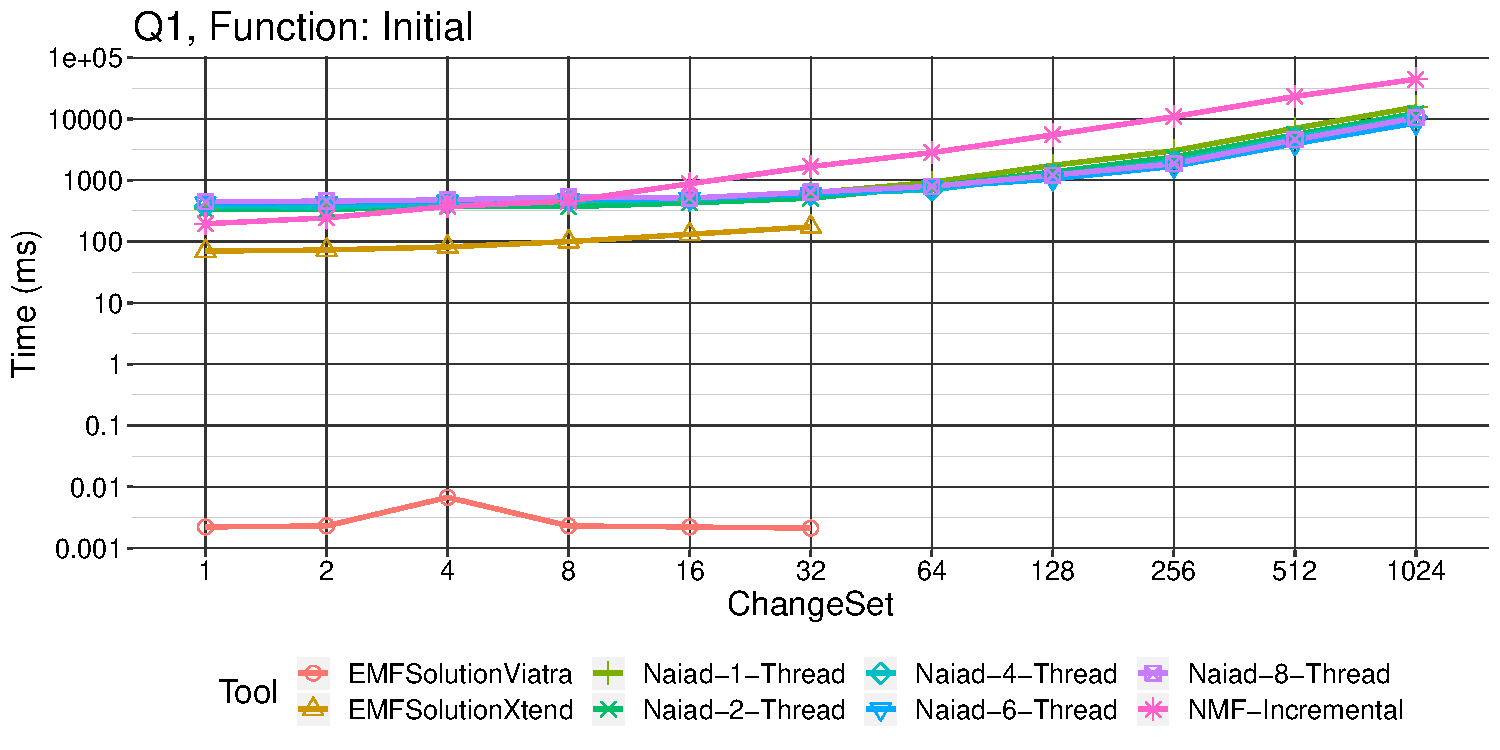
\includegraphics[width=150mm, keepaspectratio]{q1_initial}
	\caption{A Q1 lekérdezés első kiértékeléseinek válaszidői}
	\label{fig:q1_initial}
\end{figure}
\begin{figure}[ht!]
	\centering
	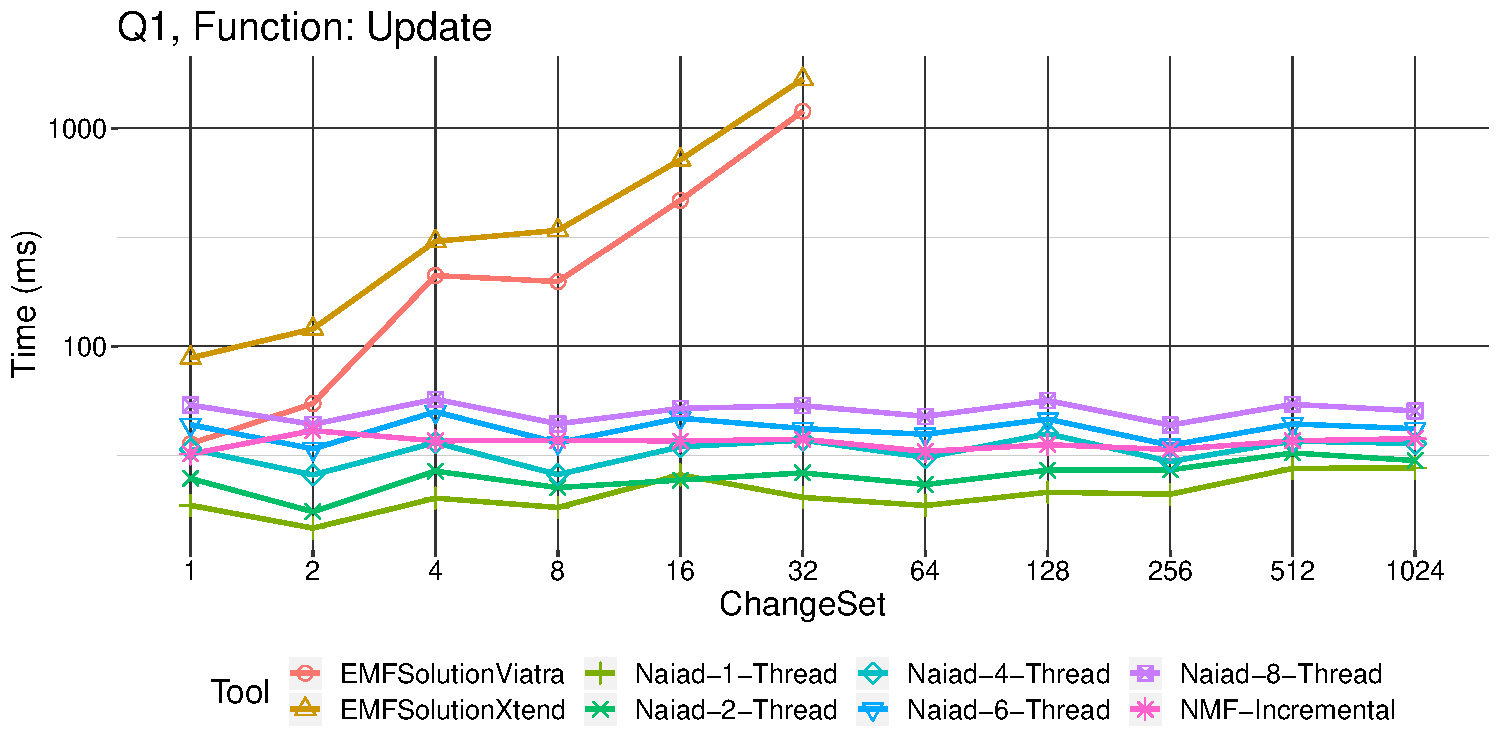
\includegraphics[width=150mm, keepaspectratio]{q1_update}
	\caption{A Q1 lekérdezés frissítések utáni kiértékeléseinek válaszidői}
	\label{fig:q1_update}
\end{figure}

\begin{table}[ht!]
	\centering
	\begin{tabular}{rrrrrrr}
		\toprule
		\multicolumn{1}{l}{Modell} & \multicolumn{1}{l}{Naiad-1} & \multicolumn{1}{l}{Naiad-2}& \multicolumn{1}{l}{Naiad-4} & \multicolumn{1}{l}{Naiad-6} & \multicolumn{1}{l}{Naiad-8}& \multicolumn{1}{l}{NMF} \\
		\midrule
		1 & 68 & 93 & 141 & 194 & 241 & 48 \\
		2 & 70 & 101 & 152 & 208 & 251 & 54 \\
		4 & 74 & 107 & 166 & 216 & 269 & 70 \\
		8 & 83 & 113 & 176 & 233 & 287 & 84 \\
		16 & 96 & 128 & 190 & 254 & 316 & 155 \\
		32 & 113 & 147 & 209 & 274 & 334 & 274 \\
		64 & 151 & 189 & 255 & 316 & 385 & 445 \\
		128 & 221 & 257 & 324 & 395 & 454 & 853 \\
		256 & 399 & 398 & 471 & 528 & 602 & 1\,408 \\
		512 & 658 & 668 & 729 & 815 & 865 & 3\,346 \\
		1\,024 & 1\,308 & 1\,285 & 1\,300 & 1\,351 & 1\,418 & 6\,424 \\
		\bottomrule
	\end{tabular}
	\caption{A Q1 lekérdezés utolsó kiértékelése utáni memóriahasználat a különböző méretű modellek és eszközök esetében MB-ban}
	\label{tab:q1-memory}
\end{table}

\paragraph{Q1 lekérdezés}

\Aref{fig:q1_initial}.~ábra mutatja a Q1 lekérdezés első kiértékeléseinek válaszidejét a modell méretének függvényében. A legszembetűnőbb eredmény a \viatra rendkívül alacsony, a többi eszköz válaszidejénél nagyjából 4 nagyságrenddel kisebb válaszideje. Ezt az okozza, hogy a \viatra már a betöltés során elkezdi a kiértékelést, és az első lekérdezésnél valószínűsíthetően már rendelkezésre álló eredményeket adja vissza. A többi eszköz közül az Xtend-es megoldás valamivel gyorsabb az Naiad és NMF alapú megoldásoknál. \Aref{fig:q1_update}.~ábrán azonban jól látszik, hogy a \viatra és az Xtend alapú megoldás is jelentősen rosszabbul teljesít, mint a Naiad és NMF alapú megoldások. Jól látható, hogy a Naiad alapú megoldások esetében a válaszidő arányos a feldolgozásra használt szálak számával. Ennek több magyarázata is lehet. Egyik lehetséges magyarázat az, hogy a számítás olyan rövid ideig tart (<100ms), hogy a többszálú feldolgozás akkora plusz komplexitást (overheadet) jelent, hogy ekkora méretű modellek esetében egyszerűen nem éri meg. Egy másik lehetséges magyarázat az, hogy egyszerűen rosszul működik a számítás elosztásáért felelős logika. Ennek eldöntéséhez nagyobb modellekre lenne szükség, ahol a számítások ideje több nagyságrenddel több időt vesz igénybe.

A Naiad teljesítményéről egyébként elmondható, hogy a vizsgált modellek esetében jól skálázódik az NMF alapú megoldással együtt, gyakorlatilag a legkisebb és legnagyobb modellen is azonos válaszidővel rendelkeznek. Érdemes megfigyelni \aref{tab:q1-memory}.~táblázaton, hogy a Naiad alapú megoldások az NMF alapú megoldáshoz képest a kisebb modellek esetén több memóriát használnak, azonban ez nagyjából a 32-es modell környékén megváltozik. A legnagyobb modell esetén az NMF alapú megoldás nagyjából ötször több memóriát használ mint a Naiad alapú megoldások. Ahogy \aref{sec:naiad-layout}.~fejezetben már kitértem rá, a \viatra és az Xtend alapú megoldások nagyjából lineárisan skálázódnak a modell méretéhez viszonyítva.

\begin{figure}[htb]
	\centering
	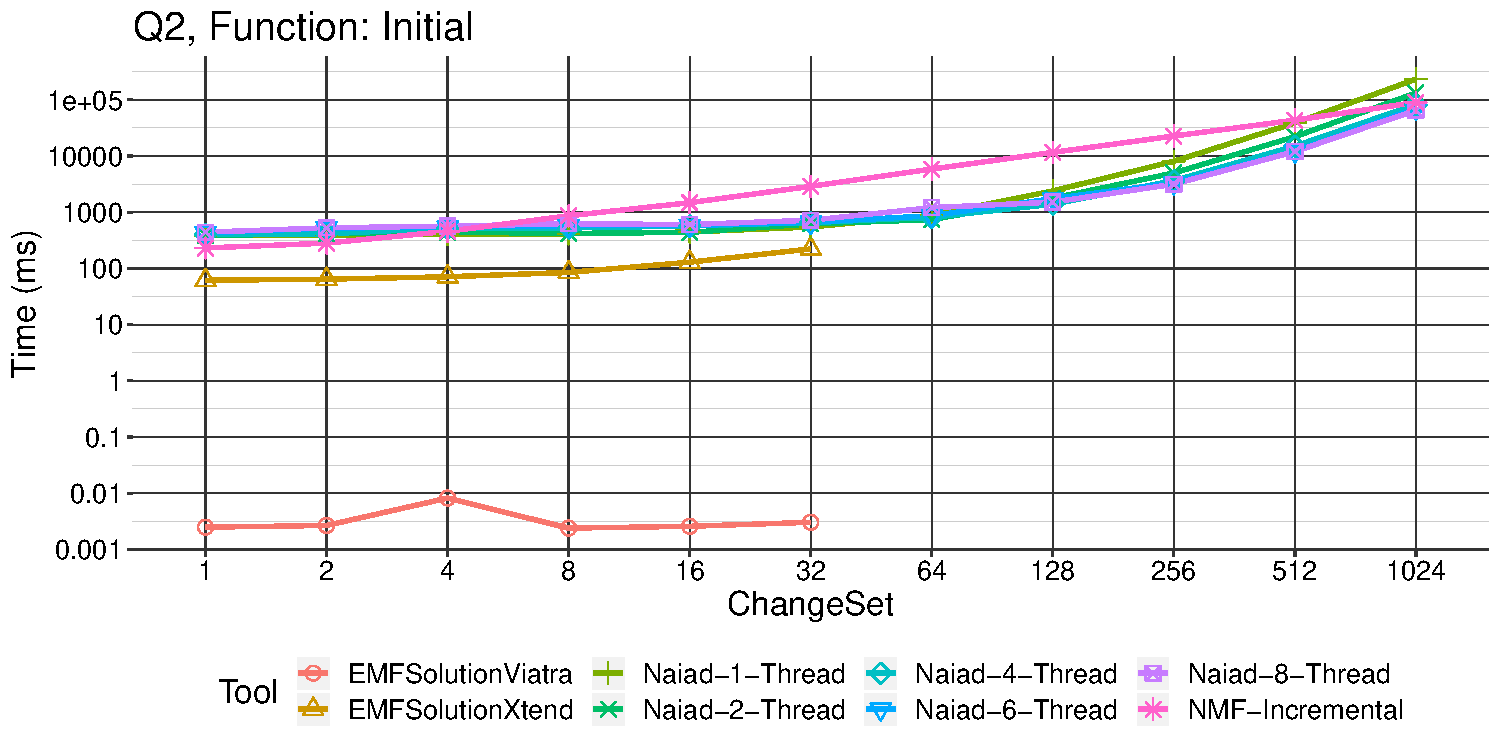
\includegraphics[width=150mm, keepaspectratio]{q2_initial}
	\caption{A Q2 lekérdezés első kiértékeléseinek válaszidői}
	\label{fig:q2_initial}
\end{figure}

\begin{figure}[htb]
	\centering
	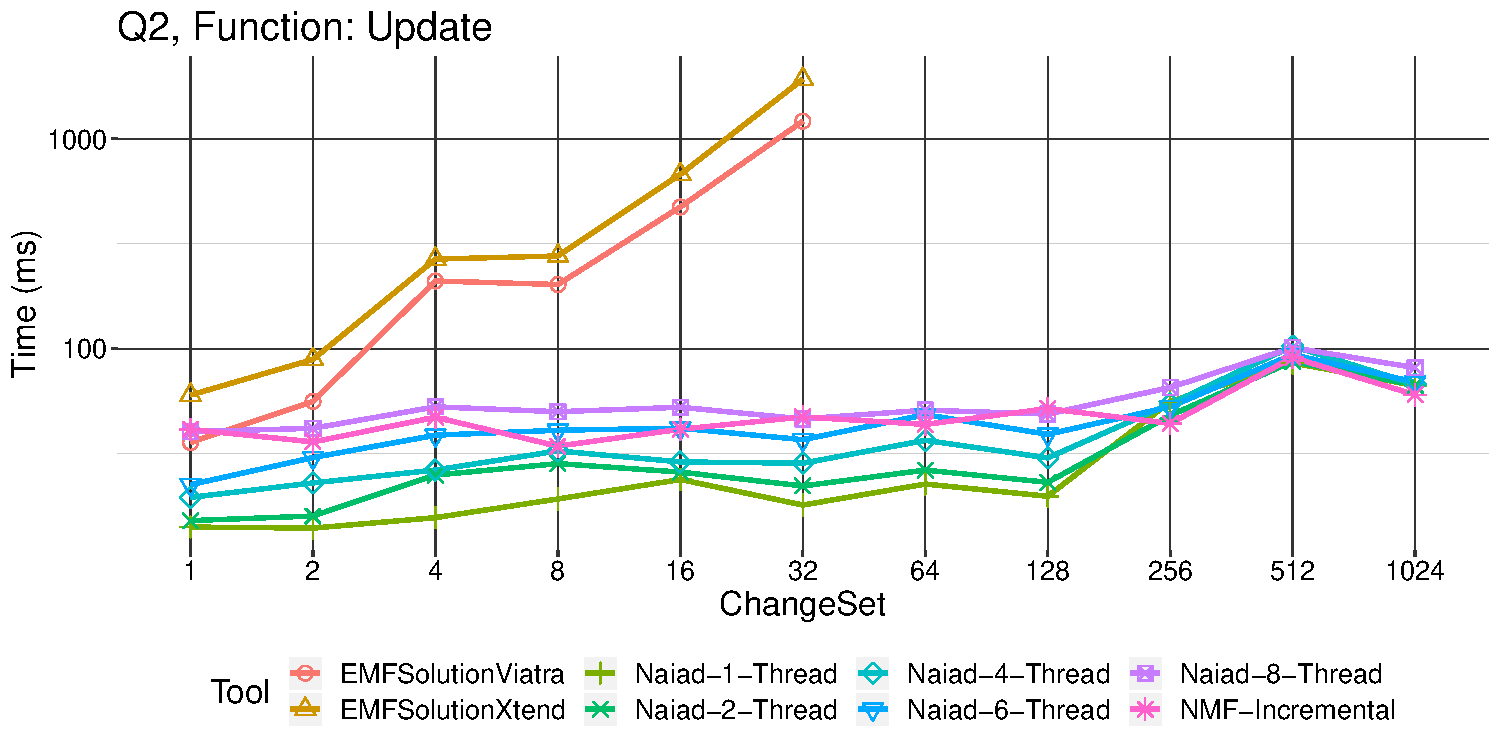
\includegraphics[width=150mm, keepaspectratio]{q2_update}
	\caption{A Q2 lekérdezés frissítések utáni kiértékeléseinek válaszidői}
	\label{fig:q2_update}
\end{figure}

\begin{table}[htb]
	\centering
	\begin{tabular}{rrrrrrr}
		\toprule
		\multicolumn{1}{l}{Modell} & \multicolumn{1}{l}{Naiad-1} & \multicolumn{1}{l}{Naiad-2}& \multicolumn{1}{l}{Naiad-4} & \multicolumn{1}{l}{Naiad-6} & \multicolumn{1}{l}{Naiad-8}& \multicolumn{1}{l}{NMF} \\
		\midrule
		1 & 60 & 71 & 88 & 114 & 123 & 47 \\
		2 & 77 & 113 & 140 & 197 & 208 & 55 \\
		4 & 84 & 127 & 186 & 252 & 300 & 74 \\
		8 & 95 & 137 & 210 & 290 & 351 & 120 \\
		16 & 107 & 155 & 243 & 335 & 414 & 199 \\
		32 & 124 & 181 & 275 & 370 & 464 & 344 \\
		64 & 168 & 224 & 330 & 444 & 555 & 681 \\
		128 & 251 & 318 & 444 & 555 & 679 & 1301 \\
		256 & 433 & 527 & 639 & 777 & 905 & 2537 \\
		512 & 929 & 997 & 1\,148 & 1\,251 & 1\,410 & 4\,882 \\
		1\,024 & 2\,281 & 2\,398 & 2\,546 & 2\,679 & 2\,836 & 9\,864 \\
		\bottomrule
	\end{tabular}
	\caption{A Q2 lekérdezés utolsó kiértékelése utáni memóriahasználat a különböző méretű modellek és eszközök esetében MB-ban}
	\label{tab:q2-memory}
\end{table}

\paragraph{Q2 lekérdezés}

\Aref{fig:q2_initial}.~ábrán látható a Q2 lekérdezés első kiértékeléseinek válaszidői a modell méretének függvényében. Az eredmények trendje nagyjából megegyezik a Q1 lekérdezés eredményével, azonban fontos észrevenni, hogy a legnagyobb modellen már egy nagyságrenddel több időt vett igénybe az első kiértékelés a Naiad és az NMF alapú megoldások esetében is. A \viatra kiugróan alacsony válaszidejének oka a Q1 lekérdezésnél leírt betöltési mechanizmus. \Aref{fig:q2_update}.~ábrán pedig a frissítések utáni kiértékelések válaszidejét tekinthetjük meg, valamint \aref{tab:q2-memory}.~táblázatban a használt memória mennyiségét. A válaszidőkről és a memóriahasználatról is nagyjából hasonló megállapítások mondhatóak el, mint a Q1 lekérdezés esetében.

Az egyetlen különböző és egyben érdekes dolog, ami a Naiad és az NMF megoldásra is jellemző a 256-os megoldástól kezdve: a válaszidők elkezdenek konvergálni, azonban nem kezd el jelentősen nőni a válaszidő. Mivel mindkét megoldás C\texttt{\#} alapú, ezért egy lehetséges magyarázat az, hogy a \emph{just-in-time} fordító (JIT) úgy értékeli a program futtatását, hogy érdemes az egyik gyakran használt kódrészletét alaposabban optimalizálni, ezért azt a kódrészletet újrafordítja, ami összemérhető nagyságrendű az egyébként nagyon alacsony válaszidővel.
